\documentclass[output=paper,colorlinks,citecolor=brown]{langscibook}
\ChapterDOI{10.5281/zenodo.19708139}
\author{Aimée Lahaussois\affiliation{Université Paris Cité and Université Sorbonne Nouvelle, CNRS, Laboratoire d'histoire des théories linguistiques, F-75013 Paris, France}}
\title{Inauspicious events and their outcomes in Thulung}
\abstract{The Thulung (Tibeto-Burman, Kiranti sub-group, Eastern Nepal) narrative corpus yields very few examples of precautioning clauses, even though such constructions are in fact fairly easy to obtain through elicitation. The precautioning construction is characterized by a) typologically unusual clause ordering, with the precautioning clause occurring before the preemptive clause; b) a negated optative form of the verb in the precautioning clause; c) subordination of the precautioning clause by means of a converbal form of the verb `to say'. Furthermore, precautioning clauses always show different subject from the pre-emptive clause, and a strong causal link across the two clauses, resulting in an avertive reading. A grammaticalization pathway is proposed for the development of this construction, originating from a lexical verb `be auspicious'. Other precautioning strategies are also found: an ‘otherwise’ (‘if not’) construction, calqued on Nepali, and a coordinated construction in which the first clause contains the precautioning event in the form of reported speech, using a finite form of the verb `to say'. 
In addition to precautioning strategies, Thulung also has an emphasis particle \textit{sɵ} which takes on an apprehensional function (but only with 2nd person S, A or P), and can be interpreted as a prohibitive in certain situations. The apprehensive domain in Thulung is much richer than initially suggested by the corpus, making use of fixed morphosyntactic constructions and coopting other language mechanisms for the expression of different types of undesirability.}

%move the following commands to the "local…" files of the master project when integrating this chapter



\IfFileExists{../localcommands.tex}{
 \addbibresource{../localbibliography.bib}
 \usepackage{tabularx,multicol}
\usepackage{url}
\urlstyle{same}

\usepackage{langsci-optional}
\usepackage{langsci-lgr}
\usepackage{langsci-gb4e}

\babelprovide[import]{hebrew}

\usepackage{paralist} %%may not be needed, currently used in questionnaire


%Siena added packages for introduction; not sure they are needed
\usepackage[normalem]{ulem}
\useunder{\uline}{\ul}{}

%from Treis:
\usepackage{listings}
\lstset{basicstyle=\ttfamily,tabsize=2,breaklines=true}

%%from Francez
% % % \usepackage{cjhebrew}
%\usepackage{tipa}  Also included by D&A, need to check with LSP whether to change it to language science tipa
\usepackage{leipzig}
%%from Dabkowski&AnderBois:

\usepackage[shortlabels]{enumitem} 
\usepackage{centernot}
\usepackage{arydshln}
\usepackage{newunicodechar}
\usepackage{csquotes}
%\let\sups\relax \usepackage{tipa} commented out on 7/3/25 Martina
% \usepackage[all]{nowidow}
\usepackage{listings} \lstset{basicstyle=\ttfamily}
\usepackage{multirow}
\usepackage{rotating}
\usepackage{pdflscape}
\usepackage{xspace}
%\usepackage{tabularx}
%\usepackage{multicol}
\usepackage{supertabular}
\usepackage{hhline}
\usepackage{bbding} %this package is for the checkmarks in Table 6 in Browne et al.

%\usepackage{qtree}
%\usepackage{tree-dvips}

\usepackage{array}
\usetikzlibrary{calc,tikzmark,matrix}
\usepgflibrary{shadings}
\usepackage{pifont}
%from Fedotov:

\usepackage{langsci-textipa}
%\usepackage{multirow}


%\usepackage{xeCJK}

%%%%%%%%%%%%%%%%%%%%%%%%%%%%%%%%%%%%%%%%%%%%%%%%%%%%
%%% EXAMPLES %%%%%%%%%%%%%%%%%%%%%%%%%%%%%%%%%%%%%%%
%%%%%%%%%%%%%%%%%%%%%%%%%%%%%%%%%%%%%%%%%%%%%%%%%%%% 

% if you want the source line of examples to be in
% italics, uncomment the following line
\renewcommand{\exfont}{\itshape}
% to add additional information to the right of
% examples, uncomment the following line

%\usepackage{langsci/styles/jambox}


%%% FOOTNOTE EXAMPLE NUMBERING
% \makeatletter
% \patchcmd{\@footnotetext}{\setcounter{fnx}{0}}{\renewcommand{\thexnumi}{\roman{xnumi}}}{}{}
% \apptocmd{\@footnotetext}{
%     \@noftnotetrue
%     \renewcommand{\thexnumi}{\arabic{xnumi}}%
% }{}{}
%
% \makeatother
\usepackage[linguistics,edges]{forest}
\usepackage{hyphenat}
\usepackage{langsci-branding}

 \makeatletter
\let\thetitle\@title
\let\theauthor\@author
\makeatother

\newcommand{\togglepaper}[1][0]{
   \bibliography{../localbibliography}
   \papernote{\scriptsize\normalfont
     \theauthor.
     \titleTemp.
    To appear in:
    Martina Faller,  Marine Vuillermet \&  Eva Schultze-Berndt (eds.). Apprehensional Constructions in a cross-linguistic perspective. Berlin: Language Science Press. [preliminary page numbering]
   }
   \pagenumbering{roman}
   \setcounter{chapter}{#1}
   \addtocounter{chapter}{-1}
}

\newbool{bookcompile}
\booltrue{bookcompile}
\newcommand{\bookorchapter}[2]{\ifbool{bookcompile}{#1}{#2}}


\newfontfamily\FedotovBoldEmptySetFont{LibertinusSerif-Italic.otf}[AutoFakeBold=2.5]
\newcommand{\FedotovBoldEmpty}{{\FedotovBoldEmptySetFont\bfseries ∅}}

%From Dabkowski&AnderBois


\let\sc\scshape
\let\rm\rmfamily
%\let\it\itshape
\let\tt\ttfamily
\let\nr\normalfont

\newcommand{\wsc}[1]{\textls[80]{\scshape#1}}

\let\textai\textit
% \let\textlc\spacedlowsmallcaps
% \let\textac\spacedallcaps
\let\textlc\textsc
\let\textac\textsc


%%%%%%%%%%%%%%%%%%%%%%%%%%%%%%%%%%%%%%%%%%%%%%%%%%%%
%%% FLAG %%%%%%%%%%%%%%%%%%%%%%%%%%%%%%%%%%%%%%%%%%%
%%%%%%%%%%%%%%%%%%%%%%%%%%%%%%%%%%%%%%%%%%%%%%%%%%%%

% \newcommand{\scott}  [1]{\textcolor{violet}{#1}}
% \newcommand{\maks}   [1]{\textcolor{blue}{#1}}
% % \newcommand{\data}   [1]{\textcolor{teal}{#1}}
% \newcommand{\new}   [1]{#1}
% \newcommand{\newnew}   [1]{\textcolor{teal}{#1}}
% \newcommand{\rev}   [1]{\textcolor{magenta}{#1}}



%%%%%%%%%%%%%%%%%%%%%%%%%%%%%%%%%%%%%%%%%%%%%%%%%%%%
%%% TABLES %%%%%%%%%%%%%%%%%%%%%%%%%%%%%%%%%%%%%%%%%
%%%%%%%%%%%%%%%%%%%%%%%%%%%%%%%%%%%%%%%%%%%%%%%%%%%%

%\newcolumntype{Y}{>{\arraybackslash}p{25.3543464286pt}} % length of L

% \newcolumntype{K}{>{\arraybackslash}p{24.25pt}}
% \newcolumntype{V}{>{\arraybackslash}p{(\textwidth/9-24pt)/2}}
%
\let\ch\relax \newcommand{\ch}[2]{\multicolumn{#1}{c}{\sc#2}}
\let\sx\relax \newcommand{\sx}[2]{\multicolumn{#1}{l}{\emph{-#2}}} % suffix
\let\su\relax \newcommand{\su}{\sx{1}} % suffix unicolumnal
\let\sd\relax \newcommand{\sd}{\sx{2}} % suffix dicolumnal
\let\cx\relax \newcommand{\cx}[2]{\multicolumn{#1}{l}{\emph{=#2}}} % clitic
\let\cu\relax \newcommand{\cu}{\cx{1}} % clitic unicolumnal
\let\cd\relax \newcommand{\cd}{\cx{2}} % suffix dicolumnal
\let\gx\relax \newcommand{\gx}[2]{\multicolumn{#1}{l}{\sc #2}} % gloss
\let\gd\relax \newcommand{\gd}{\gx{2}} % gloss dicolumnal
\let\gr\relax \newcommand{\gr}[1]{\multicolumn{2}{c}{\multirow{2}{*}{\textcolor{gray}{\sc#1}}}}
\let\db\relax \newcommand{\db}[1]{\multicolumn{2}{c}{\multirow{2}{*}{\sc#1}}}



%%%%%%%%%%%%%%%%%%%%%%%%%%%%%%%%%%%%%%%%%%%%%%%%%%%%
%%% EXAMPLES %%%%%%%%%%%%%%%%%%%%%%%%%%%%%%%%%%%%%%%
%%%%%%%%%%%%%%%%%%%%%%%%%%%%%%%%%%%%%%%%%%%%%%%%%%%%

%%% AFFIX BOUNDARY %%%%%%
% \DeclareRobustCommand{\longmn}{\textminus}
% \DeclareRobustCommand{\mn}{-}

%%% CLITIC BOUNDARY %%%%%%
% \DeclareRobustCommand{\longeq}{=}
% \makeatletter\DeclareRobustCommand{\eq}{%
%     \settowidth{\@tempdima}{-}% width of a hyphen
%     \resizebox{\@tempdima}{\height}{=}%
% }\makeatother

%%% FUZZY CLITIC %%%%%%
% \DeclareRobustCommand{\longfc}{%
%     $\overset{\text{\smash{}}}{\text{$\approx$}}$%
% }
% \makeatletter\DeclareRobustCommand{\fc}{%
%     \settowidth{\@tempdima}{-}% width of a hyphen
%     \resizebox{\@tempdima}{\height}{%
%         $\overset{\text{\smash{}}}{\text{$\approx$}}$%
%     }%
% }\makeatother

%%% REDUPLICATION %%%%%%%
% \DeclareRobustCommand{\longtl}{$\sim$}
% \makeatletter\DeclareRobustCommand{\tl}{%
%     \settowidth{\@tempdima}{-}% width of a hyphen
%     \resizebox{\@tempdima}{\height}{$\sim$}%
% }\makeatother

% \newcommand{\mn}          {\textminus}
\newcommand{\src}    [1]  {\jambox[0pt]{\rm(#1)}}
% \newcommand{\ai}     [2]  {\emph{#1} `\textsc{#2}#3'\xspace}
\newcommand{\ai}     [2]  {\emph{#1} `\textsc{#2}'\xspace}
\newcommand{\sane}   [1][]{\ai{=sa'ne}{appr}{#1}}
\newcommand{\srcn}   [1][]{\ai{kûintsû}{srcn}{#1}}
% \newcommand{\mbekane}[1][]{\ai{\eq mbe kañe}{neg.adv aux.inf}{#1}}

% \let\sc\relax \newcommand{\sc}{\normalfont\scshape}
% \let\rm\relax \newcommand{\rm}{\normalfont\rmfamily}
% \let\it\relax \newcommand{\it}{\normalfont\itfamily}

\newcommand{\lb}{{\rm[}}
\newcommand{\rb}{{\rm]}}

\newcommand{\bad}{\makebox[0pt][r]{*\,}}
\newcommand{\infel}{\makebox[0pt][r]{\#\,}}


% \newcommand{\lsqz}[1]{#1}
% \newcommand{\lsqz}[1]{\makebox[0pt][l]{#1}}

% \newcommand{\lsqu}[1]{\makebox[0pt][l]{#1}}
% \newcommand{\rsqu}[1]{\makebox[0pt][r]{#1}}
% \newcommand{\astr}{\makebox[0pt][r]{{\nr*}}}
% \newcommand{\hash}{\makebox[0pt][r]{{\nr\#}}}
% \newcommand{\qstn}{\makebox[0pt][r]{{\nr?}}}
% \newcommand{\bad}{\makebox[0pt][r]{*}}
% \newcommand{\unhappy}{\makebox[0pt][r]{\#}}


%%%%%%%%%%%%%%%%%%%%%%%%%%%%%%%%%%%%%%%%%%%%%%%%%%%%
%%% UNICODE CHARACTERS  %%%%%%%%%%%%%%%%%%%%%%%%%%%%
%%%%%%%%%%%%%%%%%%%%%%%%%%%%%%%%%%%%%%%%%%%%%%%%%%%%

\newunicodechar{⟨}{⟨}
\newunicodechar{⟩}{⟩}

\newcommand{\infix}{⟨}
\newcommand{\outfix}{⟩}



%%%%%%%%%%%%%%%%%%%%%%%%%%%%%%%%%%%%%%%%%%%%%%%%%%%%
%%% IPA %%%%%%%%%%%%%%%%%%%%%%%%%%%%%%%%%%%%%%%%%%%%
%%%%%%%%%%%%%%%%%%%%%%%%%%%%%%%%%%%%%%%%%%%%%%%%%%%%

% \newcommand{\ipa}{\textipa}

\newcommand{\sub}{\textsubscript}
% \let\super\relax \newcommand{\super}{\textsuperscript}

\newcommand{\ts}{\texttslig}
% \let\dz\relax \newcommand{\dz}{\textdzlig}
\newcommand{\tS}{\textteshlig}
\newcommand{\dZ}{\textdyoghlig}
\newcommand{\cj}{\textctc}
\newcommand{\sj}{\textctc}
\newcommand{\zj}{\textctz}
\newcommand{\tcj}{\texttctclig}
\newcommand{\tsj}{\texttctclig}
\newcommand{\dzj}{\textdctzlig}
\newcommand{\gj}{\textbardotlessj}
% \let\nj\relax \newcommand{\nj}{\textltailn}
% \newcommand{\W}{\textturnmrleg}
\newcommand{\wl}{\textturnmrleg}
% \newcommand{\1}{\ipabar{\~\i}{.5ex}{1.1}{}{}}
\newcommand{\dotlessibar}{\ipabar{\i}{.5ex}{1.1}{}{}}
\newcommand{\darkl}{\textltilde}
% \newcommand{\n}{\textsubarch}
% \newcommand{\x}{\textovercross}
\newcommand{\lowered}{\textlowering}
\newcommand{\raised}{\textraising}
\newcommand{\retracted}{\textsubbar}
\newcommand{\unreleased}{\textcorner}
% \newcommand{\syllabic}{\s}
\newcommand{\implosivet}{\texthtt}
\newcommand{\implosived}{\texthtd}
\newcommand{\implosivep}{\texthtp}
\newcommand{\implosiveb}{\texthtb}
\newcommand{\implosivek}{\texthtk}
\newcommand{\implosiveg}{\texthtg}



%%%%%%%%%%%%%%%%%%%%%%%%%%%%%%%%%%%%%%%%%%%%%%%%%%%%
%%% OTHER %%%%%%%%%%%%%%%%%%%%%%%%%%%%%%
%%%%%%%%%%%%%%%%%%%%%%%%%%%%%%%%%%%%%%%%%%%%%%%%%%%%

\newcommand{\ie}{i.\,e.\xspace}
\newcommand{\Ie}{I.\,e.\xspace}
\newcommand{\eg}{e.\,g.\xspace}
\newcommand{\Eg}{E.\,g.\xspace} 




\newcommand{\francoissource}[1]{\hfill\textnormal{{\footnotesize #1} }}
\newcommand{\E}{Ɛ\kern-1.5pt\raisebox{1pt}{̏}\kern1.5pt}
\newcommand{\ù}{{ṵ}\kern-2pt{̀}\kern2pt}
\newcommand{\ȕ}{{ṵ}\kern-2pt{̏}\kern2pt}

\newcommand{\OO}{ɔ\kern-1pt\raisebox{-1pt}{̰}\kern1pt}
\newcommand{\Ǒ}{{{ɔ̌\kern-1pt\raisebox{-.5pt}{̰}\kern1pt}}}


\newcommand{\à}{{a̰}\kern-2pt{̀}\kern2pt}
\newcommand{\ilit}[1]{#1\il{#1}}

 %% hyphenation points for line breaks
%% Normally, automatic hyphenation in LaTeX is very good
%% If a word is mis-hyphenated, add it to this file
%%
%% add information to TeX file before \begin{document} with:
%% %% hyphenation points for line breaks
%% Normally, automatic hyphenation in LaTeX is very good
%% If a word is mis-hyphenated, add it to this file
%%
%% add information to TeX file before \begin{document} with:
%% %% hyphenation points for line breaks
%% Normally, automatic hyphenation in LaTeX is very good
%% If a word is mis-hyphenated, add it to this file
%%
%% add information to TeX file before \begin{document} with:
%% \include{localhyphenation}

\hyphenation{
par-a-digm
com-ple-men-ta-tion
anaph-o-ra
Dor-drecht
Cu-shi-tic
be-ne-dic-tive
pa-ra-digms
Ethi-o-pi-an
hoch-land-ost-ku-schi-ti-schen 
Duu-raa-me
Pa-ken-dorf
Lich-ten-berk
affri-ca-te
affri-ca-tes
com-ple-ments
Eng-lish
}




\hyphenation{
par-a-digm
com-ple-men-ta-tion
anaph-o-ra
Dor-drecht
Cu-shi-tic
be-ne-dic-tive
pa-ra-digms
Ethi-o-pi-an
hoch-land-ost-ku-schi-ti-schen 
Duu-raa-me
Pa-ken-dorf
Lich-ten-berk
affri-ca-te
affri-ca-tes
com-ple-ments
Eng-lish
}




\hyphenation{
par-a-digm
com-ple-men-ta-tion
anaph-o-ra
Dor-drecht
Cu-shi-tic
be-ne-dic-tive
pa-ra-digms
Ethi-o-pi-an
hoch-land-ost-ku-schi-ti-schen 
Duu-raa-me
Pa-ken-dorf
Lich-ten-berk
affri-ca-te
affri-ca-tes
com-ple-ments
Eng-lish
}



 \boolfalse{bookcompile}
 \togglepaper[23]%%chapternumber
}{}

%The below is everything for TREES

%%Tree package finished



\begin{document}
\maketitle
%\shorttitlerunninghead{}%%use this for an abridged title in the page headers






\section{Introduction}
%\label{sec:introduction}

Considering the notable absence\footnote{\citegen{vuillermet2018a} Table 3 ``Terminology used crosslinguistically to refer to apprehensional functions'' lists languages from South America, Australia, Papunesia, North America, Eurasia (Central Siberian \ili{Yupik}) but none from South Asia.} of South Asian languages from descriptions of the apprehensional domain, this contribution aims to illustrate how \ili{Thulung}, spoken in Eastern Nepal, expresses the domain in question. As will be seen, there is indeed no dedicated morphology which ``indicates that an event will potentially occur but is undesirable, with associated pragmatics of warning or threat'' (\citealt[255]{angeloschultzeberndt2016}). \ili{Thulung} has nonetheless developed a means of expressing apprehension through a negative purpose construction, which this chapter will explore. 

\ili{Thulung} is an exclusively oral language of the \ili{Kiranti} subgroup (\ili{Sino-Tibetan}). Its verbal morphology is predominantly suffixal, with formatives used for derivation (associated motion, Aktionsart and valence changes), for the expression of arguments\footnote{The personal indexes are portmanteaux indicating person/number/clusivity and role of up to two arguments, together with tense and, when relevant, imperative mood.} and mood (optative or irrealis). Apprehension, as defined by \citet[262]{vuillermet2018a}, is a cover term that ``encompasses many different nuances of an emotion triggered by an undesirable, possible event''. By this definition, the apprehensional domain in \ili{Thulung} is expressed by means of a negative purpose construction, used to bring about the avoidance of a situation with a negative outcome. There is no morphology or construction for the expression of fear, which is instead conveyed through lexical means.\footnote{This is either through a verb `to fear', as in:
\ea \label{footnoteex}
\gll Meram-ka phʌl-mu ŋis-ta. \\
\textsc{dist.dem-erg} cut-\textsc{inf} fear-\textsc{3sg.pst} \\
\glt `He was afraid to cut [the finger].' [Miyakma-Lakpa, 127]
\z

or through the noun `fear', as in:

\ea \label{footnoteex2}
\gll A-ŋim-ka go ne a-kʌl khrep-to. \\
\textsc{1sg.poss}-fear-\textsc{instr} \textsc{1sg} \textsc{top} \textsc{1sg.poss}-face cover-\textsc{1sg>3sg.pst} \\
\glt `I covered my face in fear.' [Ghumne Pani, 97]
\z} Considering the poorly developed apprehensional domain in \ili{Thulung}, one may wonder, as did one reviewer, whether it is for good reason that languages like \ili{Thulung} are not present in typological research on apprehension, especially as, as will be seen below, there is evidence that the \ili{Thulung} negative purpose construction is calqued from (Indo-Aryan) contact language \ili{Nepali} (this is discussed in \sectref{subsec:presentation} below). It is my opinion that a better, cross-linguistic understanding of the apprehension domain necessitates input from both languages where it is well-represented, as is the case of other languages described in this volume, and those where it is a considerably more minor phenomenon, as in \ili{Thulung}, the latter providing useful insights about how a language without morphology can develop a strategy to express a category.

The structure of this contribution is as follows: in \sectref{sec:Tnegpur}, I shall describe the \ili{Thulung} negative purpose construction, proposing a development pathway based on the elements that make up the construction. I then present some related constructions, either an alternative means of expressing a similar function (the `if not' construction, in \sectref{sec:altstrategy}) or relevant in that they represent alternative grammaticalizations from a same lexical source verb (\sectref{sec:negimp}), before concluding in \sectref{lahaussois-conclusion}.


\section{The Thulung negative purpose construction}
\label{sec:Tnegpur}

According to \citet[302]{lichtenberk1995}, the precautioning function in language is made up of two subtypes: an \textit{avertive} relationship, defined by a direct causal link between the two clauses, and an \textit{`in-case'} relationship, in which precautions are taken in case the apprehension\hyp causing situation occurs but without seeking to avert it. The precautioning function is expressed through a negative purpose construction which~-- to my knowledge~-- does not have `in-case' readings.

The terminology for the semantic content of the two clauses in the negative purpose construction is that adopted throughout this volume: the apprehension-causing situation is the outcome that must be averted, expressed through what I shall call the \textit{precautioning clause}; the action taken to avoid the situation is expressed in the \textit{pre-emptive clause}. 



\subsection{Presentation and main characteristics}
\label{subsec:presentation}

The \ili{Thulung} narrative corpus which I have assembled since 1999, and which constitutes just over ten hours of interlinearized material,\footnote{Some of these annotated recordings can be found at: \url{https://pangloss.cnrs.fr/corpus/Thulung\_Rai}} yields the very low count of two examples of the negative purpose construction, seen in (\ref{ex:lah1}) and (\ref{ex:lah2}) (along with two examples of the equivalent positive purpose construction). The two other sources that exist for \ili{Thulung} diverge considerably in terms of the presence of the construction. \citet{Allen1975}, the first grammatical description of \ili{Thulung}, is accompanied by 17 pages of transcribed and glossed ``straightforward narrative texts'' (p.\ 140) (the fluent translation follows and is not part of the page count) and ten pages of a transcribed and translated (but not glossed) ``narrative text in ritual language'' (p.\ 168). Allen's corpus yields not a single instance of the negative purpose construction, nor of its positive counterpart. The second source of \ili{Thulung} narrative material is a recent \ili{Thulung} translation of the New Testament,\footnote{https://thulungmedia.com/en/thulung-bible} which yields a great number of examples of negative and positive purpose constructions matching those discussed in this contribution and illustrated in examples (\ref{ex:lah1}) and (\ref{ex:lah2}). I have found negative purpose clauses to be easy to obtain through elicitation,\footnote{By elicitation, I mean that I have gotten these constructions in response to describing a situation made up of two events, one with negative consequences and one which could help avoid the negative consequences.} and have made use of elicited material as well in the discussion presented here.



\ea \label{ex:lah1}
\gll Jakke biruwa bʌstu-ka me-po-mi-nʉ rwaksaka ur-mu ba:si. \\
small plant.species cattle-\textsc{erg} \textsc{neg}-eat-\textsc{3pl>3sg-opt} \textsc{sub} surround-\textsc{inf} must \\
\glt `So that the cattle does not eat the small plants, we must surround them (with bamboo sticks).' [verb dictionary]
\z


\ea \label{ex:lah2}
\gll Lam rem-ben-mu ʌpthero me-dʉm-nʉ rwaksaka prʌ-m-ri-m si-mu lam si-mu ɖʉmla homlowo gui thu:lu-ka bet-to-ŋa be:-mim rwak-pa lwa bu. \\
path look-\textsc{caus-inf} difficult \textsc{neg}-become.\textsc{3sg-opt} \textsc{sub} create-\textsc{1pl>3sg.pst-nmlz} die-\textsc{inf} path die-\textsc{inf} culture even.now \textsc{1di} \ili{Thulung}-\textsc{erg} do-\textsc{sim.cvb-int} do-\textsc{nmlz} say-\textsc{npst.ptcp} story be.\textsc{3sg} \\
\glt `So that it is not difficult to show [others] the path [for dealing with a corpse], we created a path for dying, and even today we \ili{Thulung} follow this ``death culture'', and this is the story of that.' [Miyakma-Lakpa, 136]
\z

The construction in (\ref{ex:lah1}) features two clauses: the precautioning clause [\textit{jakke biruwa bʌstu-ka me-po-mi-nʉ rwaksaka}], which expresses a possible negative outcome, and a pre-emptive clause [\textit{urmu ba:si}], which expresses an action to take to avoid the negative outcome. The precautioning clause contains a negated verb in the optative mood followed by the subordinator \textit{rwaksaka,} and is always a subordinate clause. The pre-emptive clause is always the main clause, which, in (\ref{ex:lah1}), contains an impersonal deontic necessity construction (see \sectref{sec:negimp} below). Note that while the form of the verb in the precautioning clause must be a negative optative, and it must be followed by subordinator \textit{rwaksaka}, there are fewer constraints on the pre-emptive clause: an impersonal deontic necessity construction is common, but so too are finite verbs, as in (\ref{ex:lah3}). 

\ea \label{ex:lah3}
\gll Tsɵttsɵ-mim-ka pi:masi me-bi-mi-nʉ rwaksaka thʌk-tʉ. \\
child-\textsc{pl-erg} fruit \textsc{neg}-beg-\textsc{3pl>3sg-opt} \textsc{sub} hide-\textsc{3sg>3sg.pst} \\
\glt `So that the children wouldn't beg for the fruit, he hid it.' [elicited]
\z

The negative optative is also found in independent clauses, as in (\ref{ex:lah4}),\footnote{\ili{Thulung} has, as discussed, an optative mood, used to express the desire that an event take place. Non-past verbs (unmarked for optative) in 1st person non-singular inclusive forms can have a hortative reading. This is contrasted, in (\ref{ex:lah4}), by translating `let's' for the hortative, and `may we' for the optative.} and expresses the speaker's desire to avoid a situation. The optative, which occurs in a complete paradigm, i.e. with all three persons, is found with both positive and negative verbs. For examples of positive optative-marked verbs, see 
(\ref{ex:lah15}) and (\ref{ex:lah16}) below. (A proposed development path for the optative marker is described in \sectref{subsec:order}.)


\ea
\label{ex:lah4}
\gll Phe:ri phe:ri hopmam dzuʈho{}-ra mi{}-grɵms-i ma ʈika ba:-mu mi-ba:si-nʉ  rwak-i. \\
again again like.this ritual.pollution\textsc{-loc}  \textsc{neg}-meet-\textsc{1pi} \textsc{conj} bindi wear-\textsc{inf} \textsc{neg}-must-\textsc{opt} say-\textsc{1pi} \\
\glt `We say ``Let's not meet again and again in this kind of ritual pollution, and may we not have to wear bindis again''.' [Life in Mukli, 185]
\z


The undesirability of the situation that is conveyed by the precautioning clause of the negative purpose construction, and which the pre-emptive action is meant to avoid, transparently comes from the negative optative form. The negative purpose construction is most often used to transmit expectations of what constitutes appropriate and inappropriate behavior, rather than to convey direct interdiction with respect to a specific action. This is probably why the pre-emptive clause often uses the impersonal deontic necessity construction, and not, as far as I can ascertain from elicitation, an imperative (this is also found to be the case in \ili{Upper Tanana Dene}, see \citealt{chapters/lovick}). \ili{Thulung} therefore does not conform to the cross-linguistic tendency, noted by \citet[24]{dixon2009}, for the clause expressing the pre-emptive action (in his terminology, the focal clause) of avertive-type constructions (subsumed within his possible consequence constructions) to contain positive or negative imperatives.

The formative \textit{rwaksaka} is also used to subordinate both expressions of direct speech or thought\footnote{This conflation of saying and thinking is common in languages of Nepal; see \citet{Noonan2006}. Also, note that all reported speech in \ili{Thulung} is expressed as direct speech.} to an utterance verb, as in (\ref{ex:lah5}), as well as other types of complement clauses, as in (\ref{ex:lah6}).

\ea
\label{ex:lah5}
\gll Khamba-nim reʈ-to-m bu rwaksaka me-sɵ-ʉ-wa. \\
Tibetan-\textsc{f} bring.up-\textsc{1sg>3sg.pst-nmlz} be.\textsc{3sg} \textsc{sub} \textsc{neg-}tell-\textsc{3sg>3sg-irr} \\
\glt `He had not told [anyone at home] that he had brought up [=married] a Tibetan woman.' [Foundation, 122]
\z

 
\ea \label{ex:lah6}
\gll Thuluŋ-ka tha:\_lwas-tʉ pʌila-ŋa oram rok-ta ma bu-mim rwaksaka tha:\_lwas-tʉ. \\
Thulung-\textsc{erg} realize-\textsc{3sg>3sg.pst} first-\textsc{int} \textsc{prox.dem} come-\textsc{3sg.pst} \textsc{conj} be-\textsc{nmlz} \textsc{sub} realize-\textsc{3sg>3sg.pst} \\
\glt `The Thulung realized, he realized that this one had arrived and stayed [there] first.' (i.e. was therefore the rightful owner of the land) [Thulung Origin, 40--41]
\z

\largerpage
 At the same time, \textit{rwaksaka} is also used, and synchronically analyzable, as an anterior converb for the verb \textit{rwa:mu}, `say', as in (\ref{ex:lah7}):


\ea \label{ex:lah7}
\gll ʌm-tsi ma ba-tsi rwak-saka mu hoʈ-dzɵl-tsi ma lʌk-tsi ʔe. \\
sleep-\textsc{2du} \textsc{conj} stay-\textsc{2du} say-\textsc{ant.cvb} fire light-\textsc{antic-2du} \textsc{conj} go-\textsc{2du} \textsc{hs} \\
\glt `Having said ``sleep and stay here'' they lit a fire and left.' [Hansel, 24]
\z

\noindent The converbal form in (\ref{ex:lah7}) is the presumed source for subordinator \textit{rwaksaka} in (\ref{ex:lah1}), (\ref{ex:lah2}), (\ref{ex:lah5}) and (\ref{ex:lah6}), similarly to what is found in many \ili{Tibeto-Burman} languages, where the grammaticalization of the verb `say' to encode ``causal, conditional, evidential, and purposive meanings'' \citep[202]{Coupe2018} is often based on a converbal form (\citealt[200--201]{Coupe2018}; \citealt{Chappell2008} for \ili{Sinitic} languages; \citealt{MaticPakendorf2013} for Siberian languages).\footnote{\citeauthor{MaticPakendorf2013} raise the possibility that Siberian \textit{non-canonical} functions for the verb `say' (among which is grammaticalization to a marker to subordinate purpose clauses) have ``historical connections with similar structures in East and Southeast Asia, the Himalayas and South Asia and the \ili{Turkic} and Turkic-influenced region spreading from Central Asia to the Balkans.'' (\citealt[358]{MaticPakendorf2013}).} This pattern is also discussed from a typological perspective by \citet[387--390]{Aikhenvald2009}, who describes a pathway for the grammaticalization of verbs of reported speech into clause-chaining devices.\footnote{\citeauthor{Aikhenvald2009} provides examples from \ili{Dolakha Newar}, \ili{Chantyal} (both spoken in Nepal) and \ili{Galo}.} The diachronic development of the subordinator probably accounts for the order of the clauses which is observed in the (negative) purpose construction and others involving material subordinated with \textit{rwaksaka}.

Interestingly, \ili{Nepali} has a strikingly similar structure to the \ili{Thulung} negative purpose construction.\footnote{The equivalent of (\ref{ex:lah8}), which was provided by Rajesh Khatiwada, is found in \ili{Thulung} in (\ref{ex:lah18}).}\footnote{The suffix \textit{-os} has been called an injunctive in some grammatical descriptions of \ili{Nepali}, and is used to ``to express a wish or desire'' (\citealt[197]{Matthews1998}). The purposive construction is also described in the same section of the grammar \citep[199]{Matthews1998}.}


\ea \label{ex:lah8} \textnormal{Nepali} \\
\gll Dza:ɖo-le nʌ-mʌr-os bhʌn-era luga lʌgai-di-ẽ. \\
cold-\textsc{instr} \textsc{neg}-die-\textsc{opt} say-\textsc{cvb} clothes wear-\textsc{appl-1sg.pst} \\
\glt `So that he would not die of cold, I dressed him.' [elicited]
\z


 The place of language contact in the use of this construction is worth considering: the constructions in \ili{Thulung} and \ili{Nepali} are close enough that it is reasonable to think of them as calques, raising the question of direction of borrowing. \ili{Thulung} is in a situation of intensive contact with \ili{Nepali}, with, to my knowledge, no remaining monolingual speakers. Evidence of borrowing from \ili{Nepali} is found throughout the language, most prominently in the lexical and syntactic domains, but with consequences for the morphosyntax as well (see \citealt{Lahaussois2003} for a contact-induced shift in the position of the ergative split within the personal pronoun system). The contact situation itself suggests that the likely direction of borrowing is from \ili{Nepali} into \ili{Thulung}, but there are other clues as well. As mentioned above, the corpus that I have made use of herein is made up of three sub-corpora: my own data, collected from 1999 onwards; some transcribed and annotated textual data from N.\ J.\ Allen, collected in the late 1960's and published in \citet{Allen1975}; and materials from recent translation efforts of the New Testament into \ili{Thulung}, available online in their Devanagari transcription. The materials collected by Allen do not contain a single occurrence of the negative purpose construction; my data contains but very few; the New Testament translation contains a great many. This could of course be due to the size of the various corpora, the New Testament translation being by far the largest of the three. But the dates are possibly also of significance, with the earlier materials showing no signs of the construction, and the more recent materials revealing its presence, suggestive of increased borrowing from \ili{Nepali}, as evidenced elsewhere in the language as well.\footnote{A third possibility is of course that the New Testament suffers from translation bias, as it was presumably based on the \ili{Nepali} version of the Bible. See \citet{Wälchli2007} for more on bias and how this affects materials, particularly parallel corpora (such as the Bible), used in linguistic studies.}


The fact that such a close mirror of the construction is found in \ili{Nepali} as well raises some profound questions about the descriptions of categories that may in fact be marginal, as suggested by one reviewer. If the \ili{Thulung} construction is calqued on the \ili{Nepali} one, then does it deserve to be described here as part of the language's apparatus for the expression of apprehension? The fact is that all of the most important elements of the construction are widely used in \ili{Thulung}: the negative optative, as well as subordination with \textit{rwaksaka}. In that sense, even if the construction itself is calqued, the elements making it up are well attested in the language (even if they in turn are possibly the result of earlier borrowing, as may be the case for subordinator \textit{rwaksaka}), and as such the construction reveals the language's ability to use what, at least synchronically, are ``native'' elements in order to express something for which a need has arisen (if we assume that the negative purpose construction is a recent phenomenon in \ili{Thulung}).

As mentioned above, \ili{Thulung} also has a positive purpose construction (again, with only two examples in my narrative corpus), which is symmetrical with the negative purpose construction described herein, consisting of an optative-marked clause, surbordinate by \textit{rwaksaka} to a main clause. It is exemplified in~(\ref{ex:lah9}):


\ea \label{ex:lah9}
\gll Omsaka pho-nʉ rwaksaka bui-ɖʌ:la jak-tʉ. \\
like.this vomit.\textsc{3sg-opt} \textsc{sub}  head-above hit-\textsc{3sg>3sg.pst} \\
\glt `So that he would vomit like this, he hit him on the head.' (in order to see what he had eaten) [Miyakma-Lakpa, 87]
\z

The only other type of purpose clause in \ili{Thulung} is one involving a motion verb,\footnote{These are of the type:
\ea \label{footnoteex3}
\gll Keʈi phʌp-ɖa lʌ:-mi. \\
girl pick.up-\textsc{purp} go-\textsc{3pl} \\
\glt `They go to pick up the girl.'
\z} a construction that only occurs in an affirmative form. There is thus only a single way to express an action carried out for negative purpose, and that is the construction described above.



\subsection{Order of clauses and grammaticalization pathway}
\label{subsec:order}

One notable characteristic of the construction is the order of clauses in the construction, which goes counter to typological tendencies: \citet[39, 48]{dixon2009} claims that for possible consequence clauses, many languages tend to move the focal clause (i.e., the pre{}-emptive clause) to the first position, giving prime importance to the expression of how to avert the negative consequence.\footnote{Note, however, that \citet[113ff]{Schmidtke-Bode2009} shows that, while VO languages have a strong preference for a purpose clause following the main clause, the data on OV languages (of which \ili{Thulung} is one) is mixed as to the ordering of clauses.} In \ili{Thulung}, the pre-emptive clause follows the precautioning clause, something which can be posited to come about from the development of the construction.

I propose the following stages for the development of the negative purpose construction:

\begin{enumerate}
    \item an optative mood marker develops from the lexical verb \textit{nʉmu} `be good, be auspicious' (henceforth glossed `be.good');
    \item a negative optative marked clause is subordinated with \textit{rwaksaka} and interpreted as a precautioning clause;
    \item the resulting precautioning clause, coupled with a main clause, yields a negative purpose construction.
\end{enumerate}

\noindent The forms that make up each stage along the pathway are still productively used. 

\subsubsection{Stage 1: Lexical verb \emph{nʉmu} to optative mood marker}
\label{subsubsec:stage1}

The lexical verb \textit{nʉmu} `be good' is illustrated in examples (\ref{ex:lah10}) and (\ref{ex:lah11}), where it appears in finite form and in participial form, respectively. The ability to occur with derivational suffixes,\footnote{The derivational suffix in (\ref{ex:lah10}) is used to express what I call \textit{liminal} Aktionsart, in other words a focus on the boundaries of the action. See \citet{Lahaussois2020b,Lahaussois2020a}.} as in (\ref{ex:lah10}), and as a participle, as in (\ref{ex:lah11}), confirms its status as a lexical verb.

\ea\label{ex:lah10}
\gll Sʉ:-ka khok-ʉ-lo wo me tsokho ɖʉ: \textbf{nʉ-le} ni. \\
who-\textsc{erg} cook-\textsc{3sg>3sg-temp} even \textsc{dem} ritually.pure beer \textbf{be.good-\textsc{lim.3sg}} indeed \\
\glt `Whoever cooks it, that ritually pure beer will end up good.' [Bungarma, 135]
\z


\ea \label{ex:lah11}
\gll Ma:ke \textbf{nʉ-pa}  khal-kam lwas-tʉ ʔe. \\
grain \textbf{be.good-\textsc{npst.ptcp}} type-\textsc{gen} see-\textsc{3sg>3sg.pst} \textsc{hs} \\
\glt `He saw a good type of grain.' (when searching for a place to establish a settlement) [Miyakma-Chandra, 115]
\z

 I propose that the verb \textit{nʉmu} `be good' develops into the optative marker through the reanalysis of two independent clauses into a mood-marked clause. In (\ref{ex:lah12}), the two independent clauses [\textit{gu dalaŋa sʌ}:] and [\textit{nʉ}] are in a paratactic relationship. 

\ea \label{ex:lah12}
\gll Gu dala-ŋa sʌ: nʉ. \\
\textsc{3sg} fast-\textsc{int} heal\textsc{.3sg} be.good.\textsc{3sg} \\
\glt `He will heal fast, that is good.' [constructed]
\z

 The two clauses in a paratactic relationship are reinterpreted as a single clause (with the prosody of the construction as it currently stands suggesting this),\footnote{Another hint is that it is written as a single word in the translation of the New Testament by native \ili{Thulung} speakers.} and \textit{nʉ} is reanalyzed as an optative mood marker, as in (\ref{ex:lah13}).


\ea \label{ex:lah13}
\gll Gu dala-ŋa sʌ:-nʉ. \\
\textsc{3sg} fast\textsc{-int} heal.\textsc{3sg}-\textsc{opt} \\
\glt `May he heal fast.' [fieldnotes]
\z

 The fact that the \textsc{3sg} non-past intransitive verb form has no overt indexation on the verb, which therefore occurs as a bare stem, results in there being no inflection marker in the space between the two finite verbs in (\ref{ex:lah12}). This could well have contributed to facilitating a reanalysis of \textit{sʌ}: as a verb root and \textit{nʉ} as a mood marker. Note that in present-day \ili{Thulung}, the optative mood marker can be suffixed directly to the verb root or to an inflected verb stem, with both forms currently accepted by some speakers, as shown in (\ref{ex:lah14}). 

\ea \label{ex:lah14}
\gll Ma:ke dzɵmka \textbf{si:-rʉ-nʉ/siʈ-nʉ} rwaksaka go biruwa dzɵmka khor-pu. \\
grain carefully \textbf{mature-\textsc{3sg>3sg.pst-opt}/mature-\textsc{opt}} \textsc{sub} \textsc{1sg} small.weeds carefully hoe-\textsc{1sg>3sg} \\
\glt `So that the grain matures nicely, I hoe the small weeds with care.' [fieldnotes]
\z

My \ili{Thulung} corpus provides a number of examples of optative mood marker \nobreakdash-\textit{nʉ}, many of which are found in recordings of incantations and prayers. Some additional illustrations are given in (\ref{ex:lah15}) and (\ref{ex:lah16}).


\ea \label{ex:lah15}
\gll Go oram-nuŋ tseŋ-si-ŋu  he: dʉm-ŋu-lo \textbf{dʉm-ŋu-nʉ} rwak-ta ʔe. \\
\textsc{1sg} \textsc{dem-soc} hang-\textsc{refl-1sg} how become-\textsc{1sg-temp} \textbf{become-\textsc{1sg-opt}} say\textsc{-3sg.pst} \textsc{hs} \\
\glt `And he said ``I will hang myself with (i.e. onto) this, and however I become, may I become like that''.' (man trying to escape from cave by grabbing onto monkey tail) [Redukpa, 107]
\z


\ea \label{ex:lah16}
\gll Bu:dzi-ŋa \textbf{me-dʉm-nʉ}  ottha tsiri-ŋa bo:-tsi gana banta ba-nna taŋma du: ba-nna. \\
shy-\textsc{int} \textbf{\textsc{neg-}become.3\textsc{sg-opt}} here tsiri.ritual-\textsc{int} do-\textsc{1du} \textsc{2sg} where be-\textsc{2sg.pst} wild.banana grove be-\textsc{2sg.pst} \\
\glt `May it not be shy, we are doing tsiriŋa here, where did you stay, did you stay in the wild banana grove?' (ritual chant in which one calls to the wild ginger to reveal itself) [Bungarma, 216]
\z


\subsubsection{Stage 2: Subordination of negative optative-marked clause}
\label{subsubsec:stage2}

Stage 1 traced the development of the optative marker. Stage 2 is that in which an optative marked clause, and specifically a negative optative marked clause, comes to be a precautioning clause, with subordinator \textit{rwaksaka}. 


In \ili{Thulung}, the subordination with \textit{rwaksaka} of a clause with an optative marked main verb yields a precautioning clause, which must then be completed by a matrix clause. Without the subordinator \textit{rwaksaka}, we simply have a clause in the optative, which can function independently (as in (\ref{ex:lah13}) or (\ref{ex:lah16})); with the subordinator, the interpretation is as a dependent precautioning clause. Thus in (\ref{ex:lah17}), which is intentionally incomplete in order to highlight the dependent status of the clause, we have what is interpreted as a precautioning clause; this needs a preemptive clause for resolution, as in (\ref{ex:lah18}) below: 


\ea \label{ex:lah17}
\gll Dzu-kka me-si:-nʉ rwaksaka \ldots \\
cold-\textsc{instr} \textsc{neg}-die.\textsc{3sg-opt} \textsc{sub} \\
\glt `So that he not die of cold, \ldots' [elicited]
\z

\subsubsection{Stage 3: Interpretation of precautioning clause coupled with appropriate main clause as a negative purpose construction.}
\label{subsubsec:stage3}

In the final stage of the proposed pathway, the combination of the precautioning clause with a main clause of appropriate semantics results in a negative purpose construction, with the main clause interpreted as the pre-emptive action which can be (or has been) taken in order to avoid the undesirable outcome expressed by the precautioning clause. As mentioned above, the main clause commonly contains an impersonal deontic necessity construction, but finite verbs are also found. Example (\ref{ex:lah18}) takes the precautioning clause from (\ref{ex:lah17}) and adds a main clause, while (\ref{ex:lah19}) is an example from the New Testament translation.\footnote{The material in (\ref{ex:lah19}) is converted from Devanagari into my transcription system, and I have added glosses and my own translation.}


\ea \label{ex:lah18}
\gll Dzu-kka me-si:-nʉ rwaksaka je phʌ-beʈ-to. \\
cold-\textsc{instr} \textsc{neg}-die.\textsc{3sg-opt} \textsc{sub} clothes wear-\textsc{caus-1sg>3sg} \\
\glt `So that he does not die of cold, I dressed him.' [elicited]
\z

   
\ea \label{ex:lah19}
\gll Mer-mim-ka paul mesinɖa me-lʌ-mi-nʉ rwaksaka sela  thʉr-so-mɖi. \\
\textsc{dist.dem-pl-erg} Paul there \textsc{neg-}go-\textsc{3sg.pol-opt} \textsc{sub} message send\textsc{-3pl>3sg.pol} \\
\glt `They sent Paul a message so that he would not go there.' [Acts 19:31]
\z

A few points should be made about the negative purpose construction resulting from the combination of the precautioning and pre-emptive clauses. The order of clauses found in \ili{Thulung}, with the pre-emptive clause following rather than preceding the precautioning clause, can be seen to come about naturally from the development of the construction: it is unsurprising in an SOV language to find complement clauses occurring before the main verb; clauses, such as precautioning clauses, which are marked with \textit{rwaksaka,} follow this order as well.

Regarding the issue of `subject' identity across clauses, \citet[133]{Schmidtke-Bode2009} has observed in his typology of purpose clauses that negative purpose clauses have a preference for ``different, i.e. non-coreferential subjects'' (36.9\% of his sample, vs.\ 5.8\% for positive purpose clauses); this contrasts with the preference of positive purpose clauses for having the same subject' (54.2\%), while negative purpose clauses only have the same subject in 10.5\% of cases. Examples collected through both elicitation and the very limited sample in my narrative corpus all have different subjects across the two clauses of the negative purpose construction. Even if the arguments of the clauses are not always explicitly expressed, as in (\ref{ex:lah18}), they are easily recoverable through indexation on the verb.\footnote{\ili{Thulung} argument indexation uses two sets of indexes, one for intransitives (glossed as the index for a single argument, `S'), and one for transitives (glossed `A>P'). In (\ref{ex:lah17}), the precautioning clause has a \textsc{3sg} S; the pre-emptive clause has a \textsc{1sg} A (and a \textsc{3sg} P), as seen from the indexation on the transitive (a causativized intransitive verb) verb \textit{phʌbeʈto.}} The occurrences of negative purpose constructions in the New Testament corpus generally concur with this same-subject tendency, but exceptions are found, such as (\ref{ex:lah20}) where the subject of both clauses is \textsc{1sg}, as can be seen from the person indexation on the verb:

\ea \label{ex:lah20}
\gll Inima nʌ me-nɵ-beʈ-pu-nʉ rwaksaka go inima-ɖa athawo tsʌkthɵ me-rok-pa mulʉ be-uto. \\
\textsc{2sg.poss} mind \textsc{neg}-hurt-\textsc{caus-1sg>3sg-opt} \textsc{sub}  \textsc{1sg} \textsc{2sg.poss-loc} or nearby \textsc{neg}-come-\textsc{npst.ptcp} decision make-\textsc{1sg>3sg.pst} \\
\glt 
`In order to not exert pain on your mind, I decided not to come to your place or  thereabouts.' [2 Corinthians 2:1]
\z

To summarize, the negative purposive construction discussed in this section is the main \ili{Thulung} construction in the apprehensional domain, i.e. used to express potential undesirable events, though it is not particularly frequently found in narratives outside translations. It is formed in an analogous manner to the positive purposive construction in \ili{Thulung}, and consists of a clause with a (negative) verb form marked with the optative and subordinated by the marker \textit{rwaksaka}. I have presented evidence that the optative mood grammaticalized from a lexical verb `be good' and the subordinator grammaticalized from an anterior converb of a quotative verb.

In the remainder of this paper, I will discuss an alternative strategy to express negative outcomes (\sectref{sec:altstrategy}), and additional functions of the optative (\sectref{sec:negimp}).




\section{Alternative strategy to express negative outcomes}
\label{sec:altstrategy}


\ili{Thulung} can also use an `if not' construction to link a pre-emptive clause to a situation expressing a potential negative outcome, as shown in (\ref{ex:lah21}). The linker between the two independent clauses, \textit{meʔema:la}, is a combination of a negative copula and a conditional marker.

\ea \label{ex:lah21}
\gll Semsʌŋ dzɵmka tsir-mu ba:si meʔema:la dzhar. \\
firewood carefully stack-\textsc{inf} must otherwise fall.\textsc{3sg} \\
\glt `Firewood must be stacked carefully; otherwise it will fall.' [verb dictionary]
\z

\noindent Note that undesirability is not expressed through this construction; it must be inferred through an evaluation of the consequence of the realization of the `if not' clause.

The same state of affairs can be expressed, with no discernible semantic differences, as a conditional with a negative protasis, as in (\ref{ex:lah22}).


\ea \label{ex:lah22}
\gll Semsʌŋ dzɵmka me-tsir-ʉ{}-wa-ma:la dzhar. \\
firewood carefully \textsc{neg-}stack-\textsc{3sg>3sg}-\textsc{irr-cond} fall\textsc{.3sg} \\
\glt `If he doesn't stack firewood carefully, it will fall.' [verb dictionary]
\z

In other words, the `if not' construction functions much like a negative conditional, with the difference that it is made up of independent clauses which are linked by \textit{meʔema:la}. The negative consequences are expressed in the second clause of both constructions, and because they are potential (rather than realized), the clause is always non-past. Another example is provided in (\ref{ex:lah23}), this time with an imperative verb in the first clause.

\ea \label{ex:lah23}
\gll ʌbʌ mal-ni ma reʈ-ni meʔema:la go gani-lai pulis-kara lʌ:-nini. \\
now search\textsc{-2pl>3sg.imp} \textsc{conj} bring-\textsc{2pl>3sg.imp} otherwise \textsc{1sg} \textsc{2pl-dat} police-\textsc{loc} take-\textsc{1sg>2pl} \\
\glt `Search and bring him, otherwise I will take you to the police.' (uttered by someone in a story whose child has been kidnapped) [Leledym, 36]
\z

The `if not' construction, seen in (\ref{ex:lah21}) and (\ref{ex:lah23}), is not considered the primary strategy for a few reasons: the negative purpose construction presented in \sectref{subsec:presentation} exhibits a stronger causal link between the two clauses, in addition to morphologically encoding undesirability through the negative optative. In the `if not' construction, the second clause factually expresses a likely outcome, should the condition expressed by the first clause not be met, and it is up to the addressee to evaluate the undesirability of the consequence of disregarding expected behavior.





\section{The negative impersonal deontic necessity construction}
\label{sec:negimp}

In addition to the pathway described above, whereby \textit{nʉmu} `be good' is the source for the optative mood marker, the same lexical verb has followed a separate grammaticalization pathway, resulting in a negative impersonal deontic necessity construction. The construction is illustrated in examples (\ref{ex:lah24}) and (\ref{ex:lah25}):


\ea \label{ex:lah24}
\gll Hapa kʌrmʌr \textbf{be-si} \textbf{menʉ}. \\
lots hard.work \textbf{do\textsc{-imper.nmlz}} \textbf{\textsc{neg.deon}} \\
\glt `One must not do lots of hard work [while pregnant].' [Childbirth, 4]
\z


\ea \label{ex:lah25}
\gll Athaldika-wo malo bʌne-mma nem-gonu ʦɵtʦɵ-mim-lai \textbf{hu:-si} \textbf{menʉ}. \\
nowadays-even just make-\textsc{pass.ptcp} house-inside child-\textsc{pl-dat} \textbf{enter-\textsc{imper.nmlz}} \textbf{\textsc{neg.deon}} \\
\glt `Even nowadays, when we make a new house, it is not acceptable for children to enter.' [Jau Khleu, 232]
\z

\noindent The bare verb root takes the impersonal nominalizer \textit{-si}, although occasionally we find an infinitive form of the verb in this construction in the place of the \textit{-si} nominalized form (an infinitive can be considered another type of nominalization). Marker \textit{-si} is assumed to be related to reflexive marker \textit{-si}, which can be used, among other functions, to express an impersonal (see \citealt{Lahaussois2016,Lahaussois2023}).

The construction stands in contrast to prohibitives (in other words, negative imperatives, which are inflected for the arguments involved): unlike the latter, it is impersonal, and is used to express recommendations against certain behaviors, generally those going against cultural norms. \ili{Thulung} prohibitives, on the other hand, refer to specific actions, undertaken by specific agents, rather than to impersonal statements about behavior. See the contrast between (\ref{ex:lah26}), the negative deontic necessity construction, and (\ref{ex:lah27}),\footnote{Examples (\ref{ex:lah26}) and (\ref{ex:lah27}) can also be contrasted with the same sentence with a negative optative:
\ea \label{footnoteex4} 
\gll Moʈorsaikʌl hapa me-onbeʈ-nʉ. \\
motorcyle lots \textsc{neg}-drive-\textsc{opt} \\
\glt `May he not drive the motorcycle too fast.' / `He shouldn't drive the motorcycle too fast.' [elicited]
\z} the prohibitive:


\ea \label{ex:lah26}
\gll Moʈorsaikʌl hapa \textbf{onbe-si} \textbf{menʉ}. \\
motorcycle lots \textbf{drive-\textsc{imper.nmlz}} \textbf{\textsc{neg.deon}} \\
\glt `One shouldn't drive a motorcycle too fast.' \\ (statement expressing opposition to a certain behavior, not directed at anyone in particular) [fieldnotes]
\z


\ea \label{ex:lah27}
\gll Moʈorsaikʌl hapa \textbf{me-onbeʈ-ni}. \\
motorcycle lots \textbf{\textsc{neg}-drive-\textsc{2pl>3sg.imp}} \\
\glt `Don't drive the motorcycle too fast!' \\
(direct interdiction, aimed at a particular person in a specific instance) [fieldnotes]
\z

 The development of the negative impersonal deontic necessity construction likely involves a transition from a negated \textsc{3sg} form of \textit{nʉmu} `be good' following a verb form nominalized with \textit{-si}, with a compositional interpretation of `V-ing is not auspicious', to a construction expressing negative deontic necessity: 

%nominalized verb (INF or \textit{-si}) + NEG-\textit{nʉ} 

%%`V-ing is not good'

%>

%`It is not good to V'

%>

%`One shouldn't V' \\
\ea \label{figure1} \textnormal{Development of the nominalized verb (\textsc{inf} or \textit{-si}) + \textsc{neg}-\textit{nʉ} into negative deontic necessity:}\\

\begin{tabular}{llll}\\[-2ex]
\textnormal{`V-ing is not good'}&
$\rightarrow$ & \textnormal{`It is not good to V'} $\rightarrow$ & \textnormal{`One shouldn't V'} \end{tabular}
\z

 This impersonal nature of the construction is reminiscent of the directive infinitive in some SAE languages. According to \citet[502]{VanOlmen2010}, ``prohibitive speech acts are more face-threatening than their positive imperative counterparts. For that reason, they also have a stronger preference for the more polite directive infinitive'' which… ``does not require a particular addressee, [and] has a weakly directive illocutionary profile''.

One factor in support of development into a full-fledged construction is that there has been phonological change: the negative marker \textit{me{\textasciitilde}mi-} is sometimes found in this construction to have assimilated to \textit{mʉ-}, resulting in a marker \textit{mʉnʉ} (and a construction V-\textit{si} \textit{mʉnʉ}). This change in the negative prefix is only found in this construction. 



%\ea \label{figure2} Two development paths from lexical verb \textit{nʉmu}
\begin{figure}[ht]

\begin{forest}
for tree={
    text width=5cm,
    edge={->}, % Make edges arrows
    align=left
%     l sep=15pt,
%     s sep=10pt
}
[{\textit{nʉmu}, `be good'},text width=3cm,
    [{Nominalized verb + negative\\
        finite form of `be good' \\
        V-\textit{mu}/V-\textit{si me-nʉ}}
        [{Impersonal negative\\
        deontic necessity \\
        V-\textit{mu}/V-\textit{si menʉ\textasciitilde mʉnʉ}\\
        `One should not V'}]
    ]
    [{Parataxis of two\\
        independent clauses\\
        V\textsubscript{finite}, \textit{nʉ}\\
        `V, and it was good'}
        [{Optative mood   V-\textit{nʉ}\\
        (and negative   Optative \textit{me}-V-\textit{nʉ})}
            [{Precautionary clause\\
            (within Avertive construction)\\
            \textit{me}-V\textsubscript{finite}/V\textsubscript{stem-nʉ} \textit{rwaksaka} \\
            `So that V doesn't happen…'}]
        ]
    ]
]
\end{forest}


% 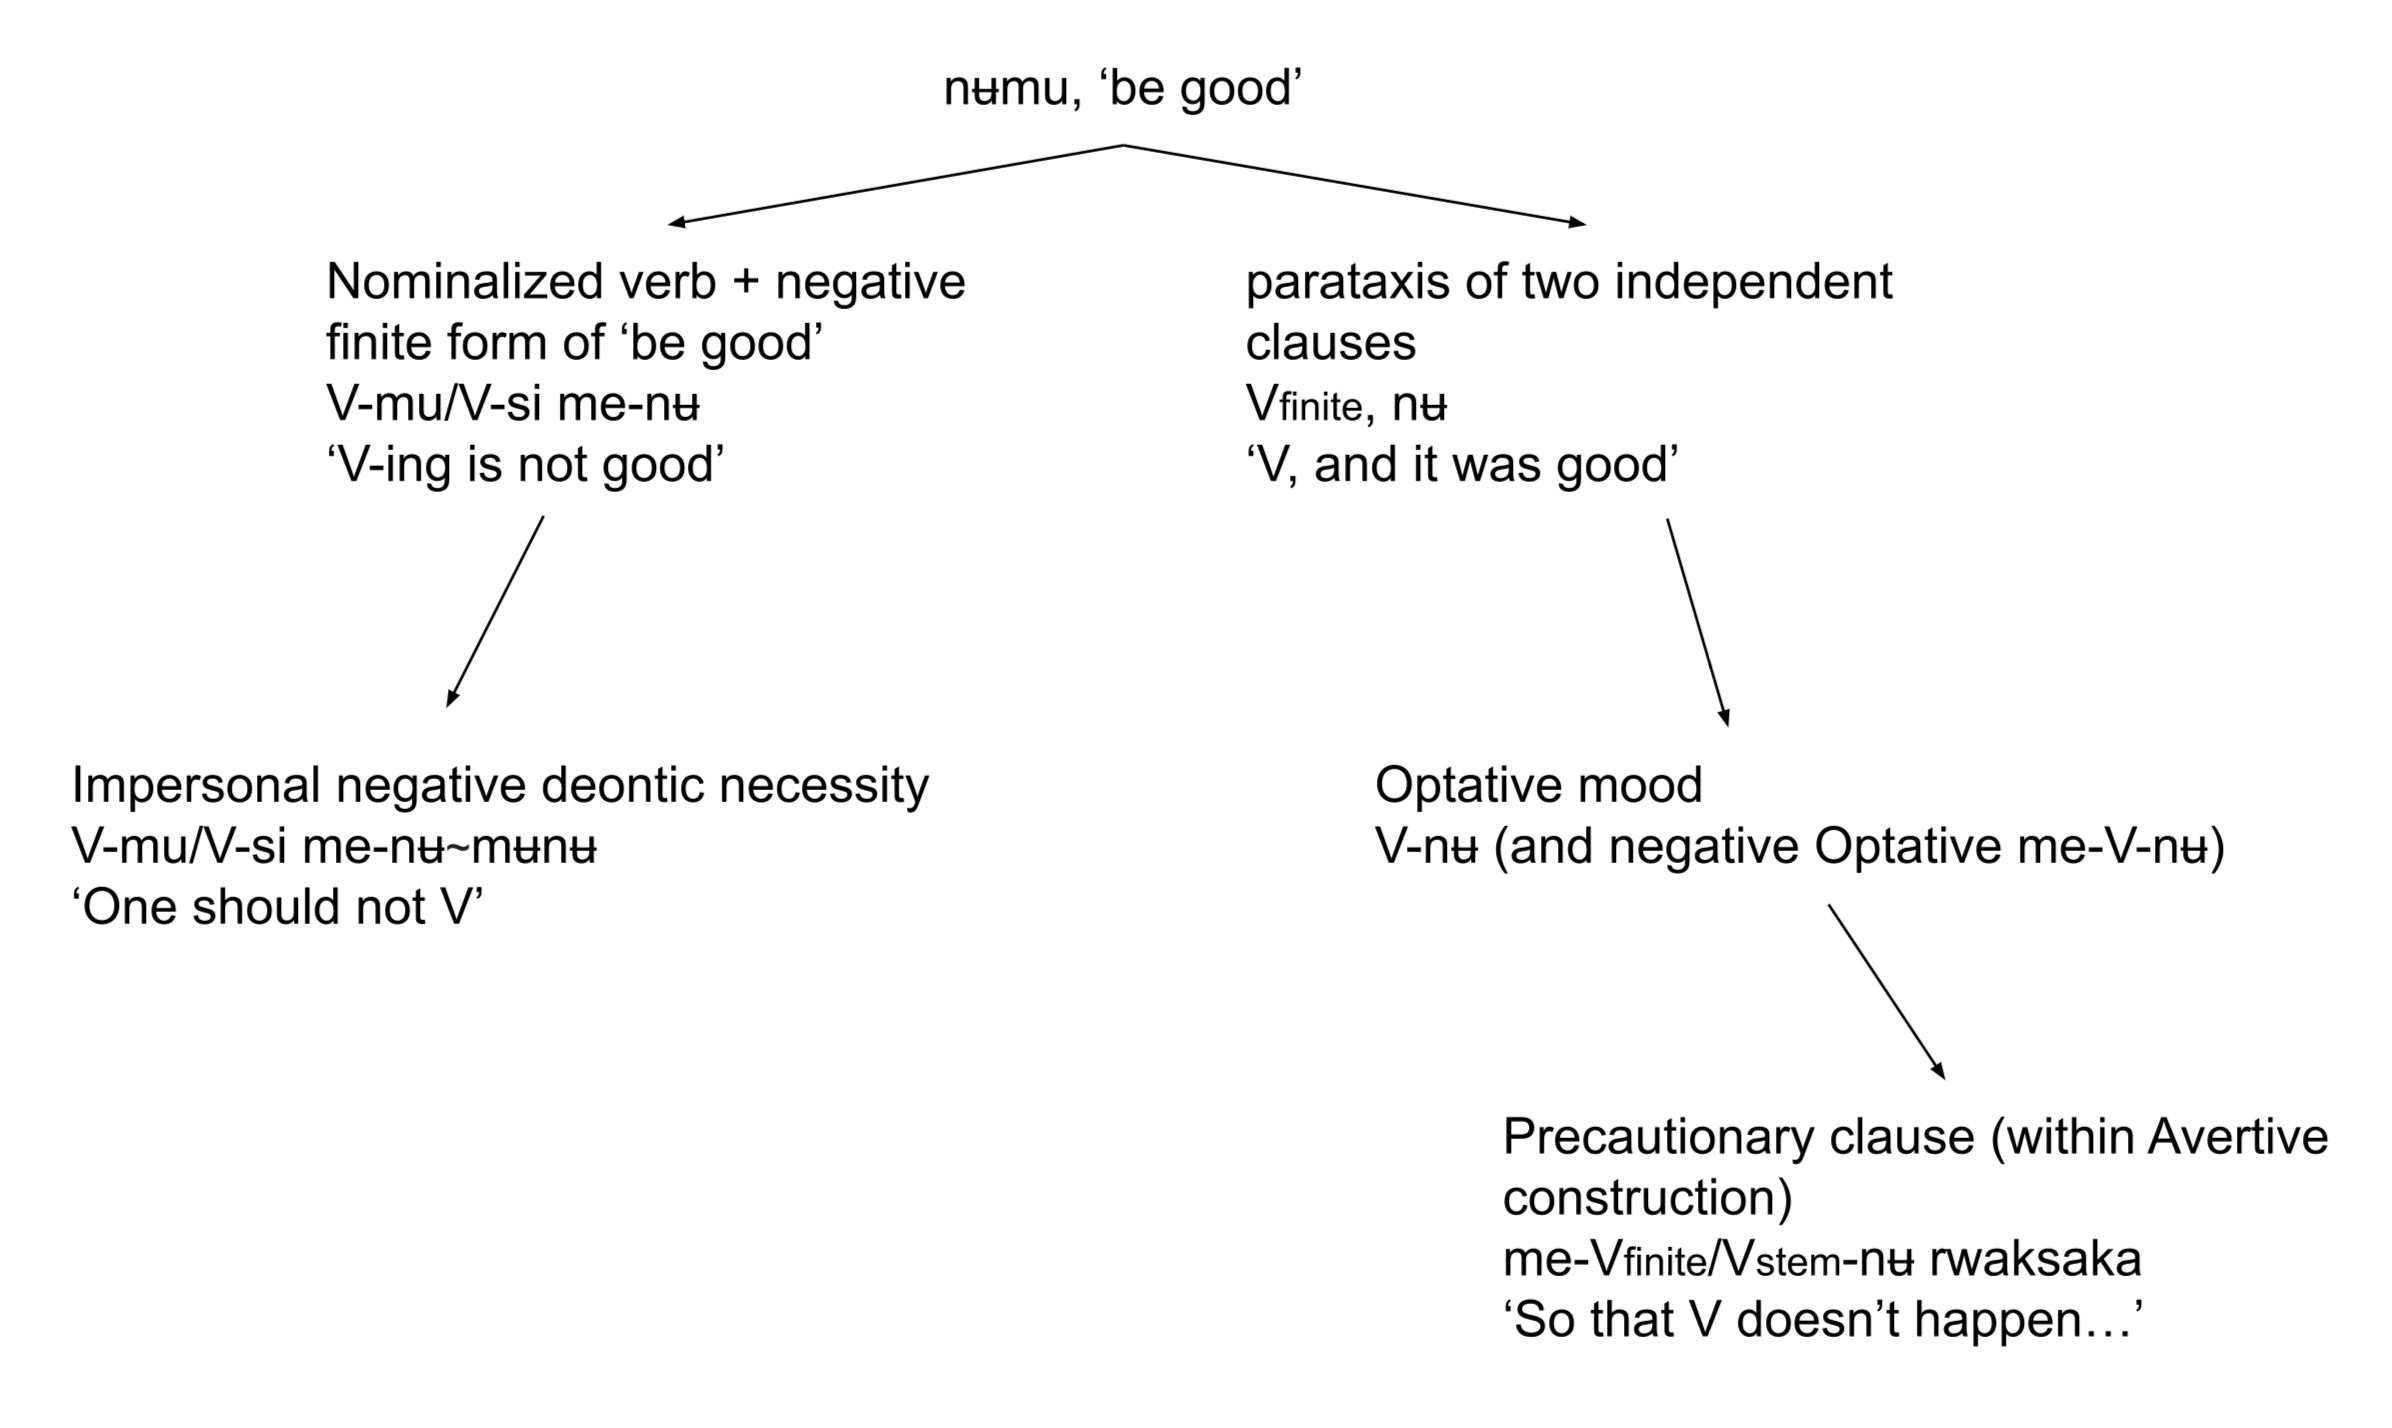
\includegraphics[width=1\textwidth]{figures/Lahaussois paths.png}
    \caption{Two development paths from lexical verb \textit{nʉmu}}
    \label{fig:Lah1}
\end{figure}

From the same source verb \textit{nʉmu} `be good', we therefore have two development pathways, resulting in an optative mood marker (which can be negative) on the one hand, and a negative deontic necessity construction on the other, as illustrated in \figref{fig:Lah1}. It is interesting that the idea of auspiciousness should feature so prominently in constructions surrounding apprehension and deontic necessity. This ties in nicely with what has been written about Rai religious practice of \textit{mundum}, namely that it ``underlies moral values and encourages the behavior that is required to uphold the order defined by the ancestors, which includes self-control, paying attention to one another, and compliance with social order'' \citep{Schlemmer2019}.



\section{Conclusion}
\label{lahaussois-conclusion}

While initial searches of the \ili{Thulung} corpus revealed no morphology dedicated to expressing apprehension, in concordance with the absence of South Asian languages in descriptions of the apprehensional domain, upon closer inspection it was found that \ili{Thulung} has nonetheless developed a strategy, in the form of the negative purpose construction. This construction results from the coopting of morphology with other functions, namely a negative optative verb form and a subordinator, in order to yield a precautioning clause which combines with a main clause expressing a pre-emptive action to avert the undesired outcome. This contribution has attempted to provide some empirical data on how the apprehensional domain is expressed in \ili{Thulung}.

\section*{Acknowledgements}

I wish to thank the editors for bringing such an interesting research topic to the attention of a wider group of linguists, and for their hard work and energy in assembling and editing the present volume. I also gratefully acknowledge the very helpful and insightful comments and suggestions of two anonymous reviewers.



\section*{Abbreviations}
\begin{tabularx}{.55\textwidth}{@{}lQ@{}}
\textsc{1, 2, 3} & first, second, third person \\
\textsc{add} & additive (`also') \\
A & agent argument\\
\textsc{ant.cvb} & anterior converb \\
\textsc{antic} & anticipatory Aktionsart (telic) \\
\textsc{appl} & applicative \\
\textsc{caus} & causative \\
\textsc{cond} & conditional \\
\textsc{conj} & conjunction \\
\textsc{dat} & dative \\
\textsc{dem} & demonstrative \\
\textsc{dist} & distal \\
\textsc{du} & dual \\
\textsc{erg} & ergative \\
\textsc{f} & feminine \\
\textsc{gen} & genitive \\
\textsc{hs} & hearsay \\
\textsc{imp} & imperative \\
\textsc{imper.nmlz} & impersonal nominalizer\\
\textsc{inf} & infinitive \\
\textsc{instr} & instrumental \\
\textsc{int} & intensifier \\
\textsc{irr} & irrealis \\
\textsc{lim} & liminal Aktionsart (telic) \\
\textsc{loc} & locative \\
\textsc{neg} & negative\\
\textsc{neg.deon} & negative deontic \\\end{tabularx}%
\begin{tabularx}{.44\textwidth}{@{}lQ@{}}
\textsc{nmlz} & nominalizer \\
\textsc{npst.ptcp} & non-past participle \\
\textsc{opt} & optative \\
\textsc{pass} & passive \\
\textsc{P} & patient argument\\
\textsc{pi} & plural inclusive \\
\textsc{pl} & plural \\
\textsc{pol} & polite (for personal pronouns) \\
\textsc{poss} & possessive \\
\textsc{prox} & proximal \\
\textsc{pst} & past \\
\textsc{ptcp} & participle \\
\textsc{purp} & purposive \\
\textsc{refl} & reflexive \\
SAE & Standard Average Eureopean\\
S & subject of intransitive verb\\
\textsc{sg} & singular \\
\textsc{sim.cvb} & simultaneous converb \\
\textsc{soc} & sociative \\
\textsc{sub} & subordinator \\
\textsc{temp} & temporal sequencer \\
\textsc{top} & topic \\
V & verb\\\\
\end{tabularx}

%\textsc{} &  \\



\printbibliography[heading=subbibliography,notkeyword=this]
\end{document}
